% INTRODUCTION
Marine aggregates are randomly formed particles composed of organic and inorganic matters, such as phytoplankton, detritus, sediment, and fecal pellets \cite{jackson_simulation_1989}. Since these components stick together arbitrarily, a marine aggregates is often shown a fractal structure. 
These marine aggregates take in carbon dioxide (CO$_2$) during photosynthesis near the surface ocean and carry the dissolved carbon to the deep ocean. 
% The ocean absorbs $40 \%$ of the anthropogenically produced carbon dioxide (CO$_2$) from the atmosphere \cite{omand_sinking_2020}. 
This process removes CO$_2$ from the atmospheric carbon cycle \cite{honjo_understanding_2014}, and plays a role in regulating atmospheric CO$_2$ and climate changes which is one of the most significant environmental problems we face today. 
 \par
 It has been observed that larger sinking aggregates tend to accumulate in thin layers where the ambient fluid is density stratified \cite{alldredge_occurrence_2002}.The highly concentratedthin layers become biological hotspots for bacterial activity and animal feeding. It is ecologically important to understand the marine aggregates dynamics as they delay in settling.
\par
We consider flow around aggregates in the low Reynolds number regime, which is applicable for approximately the smallest 30\% of marine aggregates \cite{alldredge_situ_1988}. Flow in this regime is governed by the Stokes equations, which allows solutions to be found via boundary integral methods \cite{pozrikidis_boundary_1992}. Such methods  have been implemented in several different contexts, typically via a combination of analytical integration near the singularities that arise and quadrature methods away from the singularities, see \cite{pozrikidis_boundary_1992} for a review. Boundary integral methods
are particularly well suited to computations of flow around complex solids  \cite{zinchenko_boundary-integral_2006}  as velocity and forces may be expressed in terms of an integral over the boundary of the object. 
They have also recently been combined with other methods, for example to capture interactions between fluids and elastic solids \cite{bao_immersed_2017} and stochastic fluctuations in suspensions \cite{bao_fluctuating_2018}.
Here, we form aggregates using cubic particles, which results in a simple boundary over which the resulting integrals can be computed analytically, as described in chapter 2.
This has the advantage of avoiding numerical singularities on the boundary, which otherwise require regularization \cite{cortez_method_2001} or specialized numerical methods such as high-order product Nystr\"{o}m methods \cite{atkinson_numerical_1997, delves_computational_1985}, adaptive sub-domain integration \cite{chan_second-order_1992},
or  nearest-neighbor discretization of the regularized Stokeslet boundary integral equation \cite{smith_nearest-neighbour_2018}.
 We introduce a novel implementation of boundary integral methods which is both simple  and well-behaved numerically. 
Details of this new methodology, along with its validation are presented in Section \ref{sec:numerical}. We compare two approaches, using a single-layer and double-layer integral representation of the velocity \cite{pozrikidis_boundary_1992, power_second_1987, ingber_comparison_1999}, and determine which is the most suitable for fluid flow simulations around marine aggregates with this new method.


 \par
Our research is centered on computing the velocity field around settling marine aggregates and the forces acting on them. We do so using boundary integral equation (BIE) formulations. We construct marine aggregates using cubes to capture their fractal shape, as shown in Figure \ref{fig_cube10}. 
\begin{figure}[ht]
	\begin{center}
		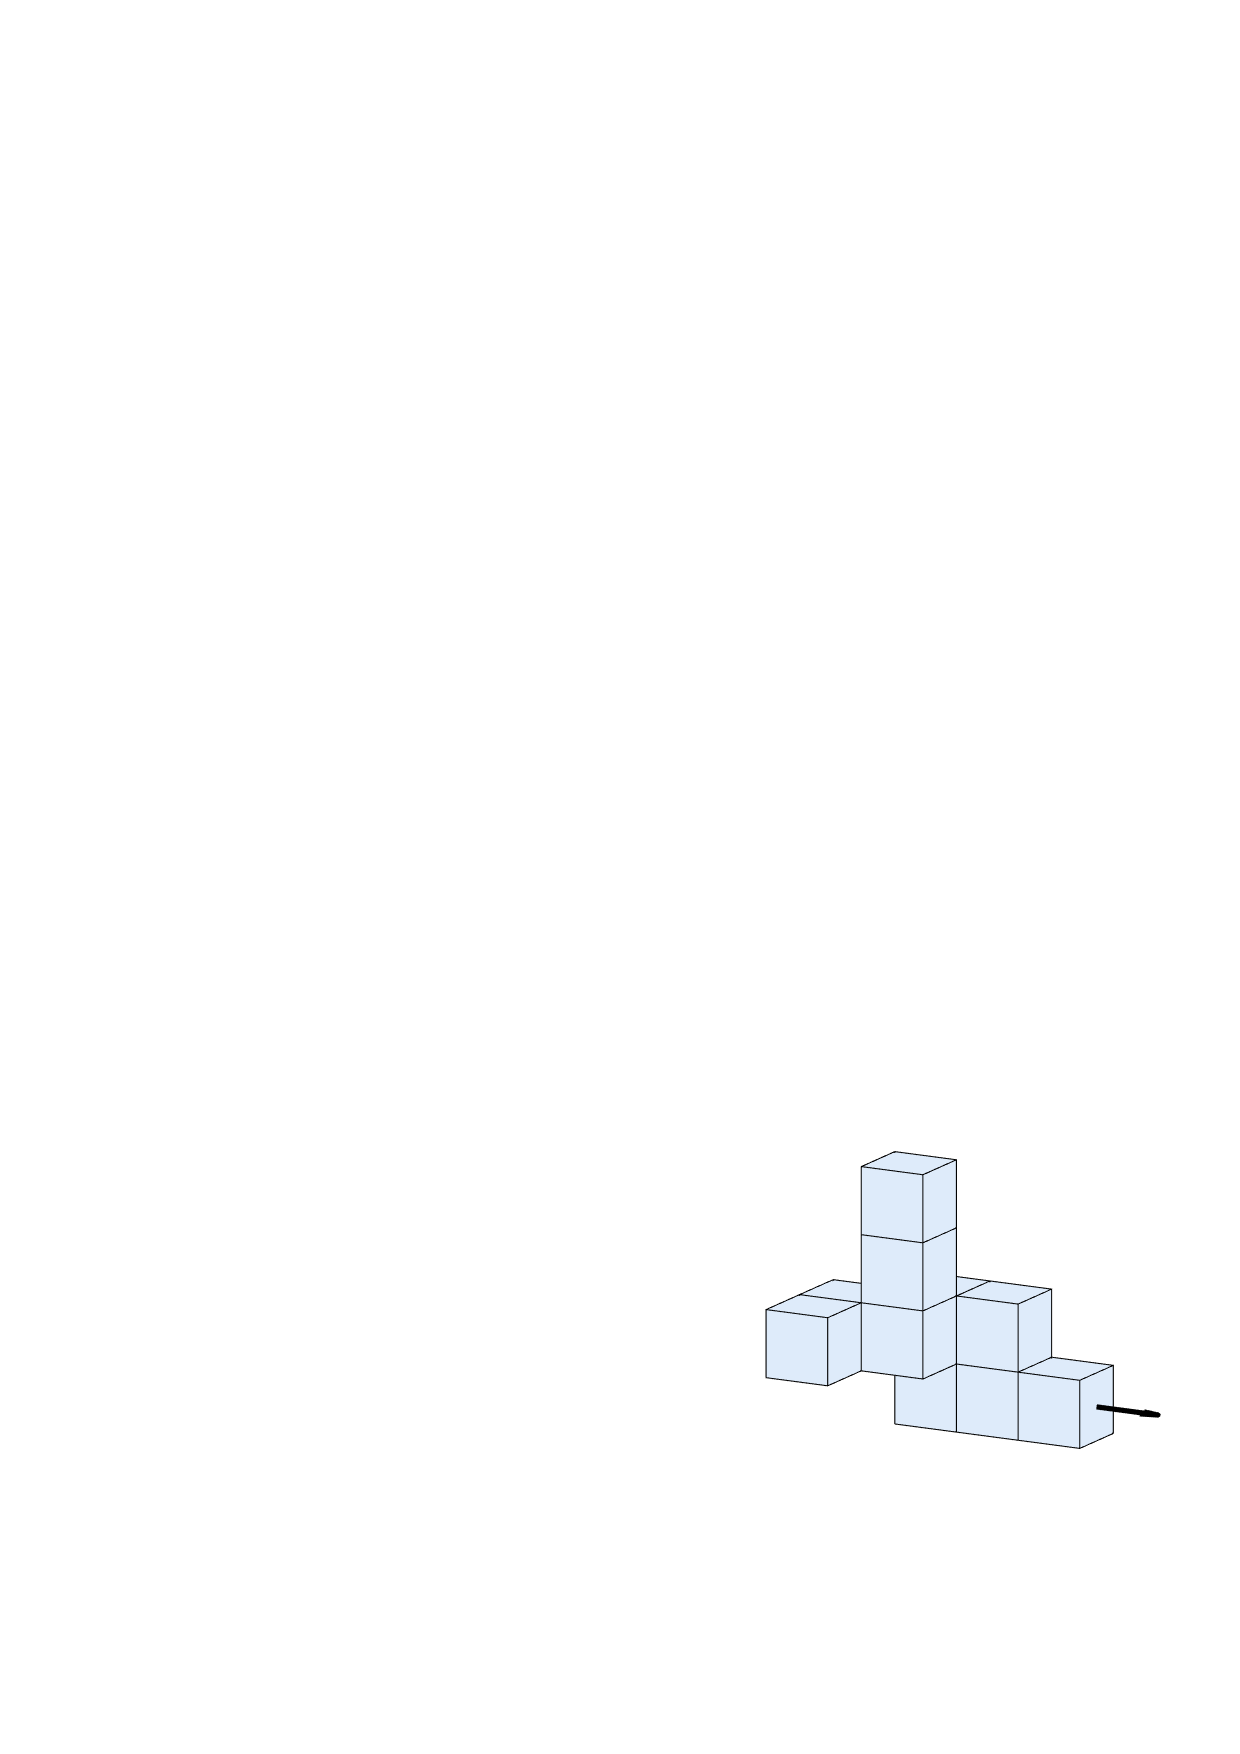
\includegraphics[scale=0.25]{figures/fig_sample_cube10.pdf}
	\end{center}
	\caption{Example aggregate model with 10 cubes. We denote $S$ as the aggregate boundary surface and $\hat{n}$ as its normal. The vectors $\vec{x}$ and $\vec{y}$ are points on and outside of $S$. The solid lines represent the fluid domain boundaries.}
	\label{fig_cube10}
\end{figure}

\section{Fluid momentum equations}
To describe the incompressible fluid motion that takes place around marine aggregatess, we consider the Navier-Stokes equations,
\begin{align}
\nabla \cdot \vec{u} = 0 
\label{eq_conserv_mass} \\
\rho 
\left( 
   \frac{\partial \vec{u}}{\partial t} + \vec{u}\cdot \nabla \vec{u}
\right)
  = \nabla \cdot \bar{\bar{\sigma}} +  \rho  \vec{g} ,
\label{eq_momentum_NS}
\end{align}
where $ \rho$ is fluid density (constant) and $\vec{u}, \ \vec{g}$ are fluid velocity and gravity vectors, respectively.
The first equation (\ref{eq_conserv_mass}) shows the conservation of mass and the equation (\ref{eq_momentum_NS}) describes the momentum conservation. 
We also introduce the stress tensor, $\bar{\bar{\sigma}}$ as 
\begin{equation}
   \bar{\bar{\sigma}} = -P \bar{\bar{I}} + {\tilde{\mu}} {\bm D},
   \label{eq_stress_tensor}
\end{equation}
where $P$ is fluid pressure and ${\tilde{\mu}}$ is fluid viscosity. Here, ${\bm D}$ is the symmetric strain rate tensor,
\begin{equation}
   \boldsymbol{D} = \frac{1}{2} \left( \nabla \vec{u} + (\nabla  \vec{u})^T \right).
   \label{eq_strain_rate}
   \end{equation}
Since seawater is Newtonian fluid, following the Newton's law of viscosity, the strain rate (\ref{eq_strain_rate}) becomes $\nabla \vec{u}$. This implies that we can re-write the momentum equation (\ref{eq_momentum_NS}) as
\begin{equation}
  \rho \left( 
   \frac{\partial \vec{u}}{\partial t} + \vec{u}\cdot \nabla \vec{u}
\right)
  = -\nabla P  + {\tilde{\mu}} \nabla^2 \vec{u}+  \rho  \vec{g} 
  \label{eq_stokes_momentum}
\end{equation}
For a typical seawater, it is reasonable to say $\rho \approx 1025 \text{kg/m}^3$ and ${\tilde{\mu}} = 1.2 \times 10^{-3}\text{kg}/\text{ms}$.
Also, the gravitaty vector is $\vec{g} = - g\hat{k} \approx -9.8$m/$s^2 \times (0,0,1)$ where $\hat{k}$ points in the vertical direction (upward). 
\par
 The momentum equation (\ref{eq_momentum_NS}) can be linearized for flows where inertial effects are small. 
To estimate the size of the main forces at play, we consider a radius of marine aggregate, $R_a \approx 5 \times 10^{-5}$(m) and the reference Stokes settling speed of an aggregate,
\begin{equation}
    U_s =  \frac{gR_a^2}{{\tilde{\mu}}} (\rho_a-\rho) \approx 3.8 \times 10^{-4} ({\text{m/s}}),
	\label{eq_U_s}
\end{equation}
where $\rho_a \approx 1400\text{kg/m}^3$ is the aggregate mass density. 
When we non-dimensionalize the momentum equation using the length scale, $R_a$ and velocity, $U_s$, we can obtain the following equation:
\begin{equation}
	\left(\frac{\rho U_s R_a}{{\tilde{\mu}}} \right) 
   \left( 
   \frac{\partial \vec{u}'}{\partial t'} + \vec{u}'\cdot \nabla' \vec{u}'
\right)
 = {\nabla'}^2 \vec{u}' - \nabla' P' +  \vec{g}',
 \label{eq_NS_moment_noD}
\end{equation}
where we find and compute the Reynolds number (Re),
\begin{equation}
	\text{Re} = \frac{\rho U_s R_a}{{\tilde{\mu}}} \approx 10^{-2}
	\ll 1.
   \label{eq_Re}
\end{equation}
Note that we use the prime symbol to represent a dimensionless value.
Since we have fairly small Reynolds number, we may neglect the inertial effects, limiting the left-hand side of equation (\ref{eq_NS_moment_noD}) to zero,
\begin{equation}
   {\nabla'}^2 \vec{u}' - \nabla' P' +  \vec{g}' = 0.
\end{equation}
In this thesis, we therefore consider the following Stokes equations, writing back with dimensions, to describe the fluid flow around the settling aggregates,
 \begin{align}
	\nabla \cdot \vec{u}  = 0  
	% \label{eq_conti2}
	\nonumber \\
	{\tilde{\mu}} \nabla^2 \vec{u}    - \nabla P\ + \rho  \vec{g} = 0.
	\label{eq_stokes2}
\end{align}
The solutions of the system of equations are the fluid velocity, $\vec{u}$, and pressure, $P$. In general, pressure does not induce motion. We see the pressure at rest, denoted as $P_s$, contains the pressure of gravity,  $P_s(\vec{y}) = \rho \vec{g} \cdot \vec{y}$, where $\vec{y} \in \mathbb{R}^3$ is a point in the fluid. Using this static pressure term, we introduce the dynamic pressure $P_d$, defined as 
\begin{equation}
   P_d(\vec{y}) = P(\vec{y}) - P_s(\vec{y}) = P(\vec{y}) - \rho \vec{g} \cdot \vec{y}.
   \label{eq_def_Pd}
\end{equation}
By substituting the expression (\ref{eq_def_Pd}), we obtain
\begin{align}
	\nabla \cdot \vec{u}  = 0  
	% \label{eq_conti2}
	\nonumber \\
	{\tilde{\mu}} \nabla^2 \vec{u}    - \nabla P_d = 0.
	\label{eq_stokes3}
\end{align}
In our simulation, we focus on the velocity field and hydrodynamic forces around the marine aggregate model. 
%===SECTION 2.2=========================================
\section{Boundary integral equation (BIE) formulations} 
For our simulations, we consider a large fluid domain compared to the size of an aggregate, having zero fluid velocity at infinity. We also treat our aggregate surface as a solid. Although marine aggregates are porous, the solid boundary condition is reasonable to apply due to their low permeability. 
% These conditions allow us to eliminate one of the integrals. The detailed derivation is provided in section 2. 
This condition prevents a flow through the aggregate, acting like a solid particle. For this reason, any flow inside of the aggregate is neglected in the remainder of this thesis.  
\par
For a general surface S, the velocity $\vec{u}$ at a point $\vec{y}\in \mathbb{R}^3$ exterior to the surface may generally be expressed using the representation formula \cite{pozrikidis_boundary_1992}
% around a solid object is expressed, using the stress vector, $\vec{f}$, 
\begin{equation}
   \vec{u}(\vec{y}) =
	- \frac{1}{8 \pi {\tilde{\mu}}} \int_S  \vec{f}(\vec{x}) \cdot \bar{\bar{G}}(\vec{x},\vec{y}) \ \text{d}S(\vec{x}) 
+ \frac{1}{8 \pi} \int_S
\vec{u}(\vec{x}) \cdot  \bar{\bar{K}}(\vec{x},\vec{y})  
\cdot \hat{n} ( \vec{x})
\ \text{d}S(\vec{x}),
\label{eq_BIE}
\end{equation}
% where  $\vec{f}(\vec{x})$ is the stress vector that describes a point force at $\vec{x} \in S$. 
where the integral is taken over points $\vec{x}$ on the surface $S$.
The kernel $\bar{\bar{G}}(\vec{x},\vec{x}_0)$ is the Green's function of the Stokes equations at any point $\vec{y}$, that is the {\textit{Stokeslet}}, in the domain for a point-source located at $\vec{x}$,
\begin{align}
  \bar{\bar{G}}(\vec{x},\vec{y}) =   
  \frac{\bar{\bar{I}}}{||\vec{x}-\vec{y}||} + \frac{(\vec{x}-\vec{y})(\vec{x}-\vec{y})}{||\vec{x}-\vec{y}||^3}.
  \label{eq_stokeslet}
  \end{align}
  The kernel  $\bar{\bar{K}}(\vec{x},\vec{y})$ is the stress tensor associated to this fundamental solution, named {\textit{Stresslet}},
  %
  \begin{align}
  \bar{\bar{K}}(\vec{x},\vec{y}) = 
  -6\frac{(\vec{x}-\vec{y})(\vec{x}-\vec{y}) (\vec{x}-\vec{y})}{||\vec{x}-\vec{y}||^5},
  \label{eq_stresslet}
  \end{align}
where $\| \cdot \|$ is the $L^2$ norm. 
The first integral distribution on the right-hand side of equation (\ref{eq_BIE}) is called the \textit{single-layer potential} and the second one is called the \textit{double-layer potential}. 
To compute the velocity at a point on the surface $S$, i.e., $ \vec{x}_s \in S$, we use 
\begin{equation}
   \vec{u}(\vec{x}_s) = - \frac{1}{4 \pi {\tilde{\mu}}} \int_S  \vec{f}(\vec{x}) \cdot \bar{\bar{G}}(\vec{x},\vec{x}_s) \ \text{d}S(\vec{x}) 
+ \frac{1}{4 \pi} 
\int_S
\vec{u}(\vec{x}) \cdot  \bar{\bar{K}}(\vec{x},\vec{x}_s)  
\cdot \hat{n} ( \vec{x})
\ \text{d}S(\vec{x}).
\label{eq_BIE_onS}
\end{equation}
Also, $\vec{f}(\vec{x})$ is the generally unknown  stress vector, or traction, on the surface, and $\vec{u}(\vec{x})$ is the, generally unknown, velocity on the surface $S$. 
When $S$ is the boundary of a solid object, in our case an aggregate, the general representation formula may be simplified in two different ways, depending on the fluid domain characteristics and/or type of the object's surface. We will introduce those two formulae in chapter 2. 


\section{Non-Newtonian fluid}
% Main difference between Newtonian vs Non-Newtonian. Explain the yield stress. Basic idea of rheology, and importnace of the secondary flow we want to capture.
In the last part of this thesis, we will turn our attention to non-Newtonian fluids. This topic is added to my thesis as an extension of one summer internship at the Lawrence Berkeley National Lab in 2022, under the guidance of Dr. Ishan Srivastava. 
\par
A non-Newtonian fluid shows many interesting behaviors quite different than Newtonian fluids. It has variable viscosity that changes the state of a fluid depending on flow conditions, i.e., the viscosity term,${\tilde{\mu}}$ in the stress tensor (\ref{eq_stress_tensor}) is not constant; rather it is a function of the shear rate ($\dot{\gamma}$), i.e., $\mu(\dot{\gamma})$, where
  $ \dot{\gamma} = \left| 
   {\boldsymbol{D}}
   \right|.
$
Due to this varying viscosity, the constitutive behavior of non-Newtonian fluids is highly complex. They show intriguing phenomena such as shear thickening, shear thinning, jamming, shear banding, and normal stress differences. This broad class of fluids encompasses various materials of industrial and natural importance, such as granular fluids, polymeric fluids, gels, and suspensions. Complex fluids exhibit two phases as responses to applied stress. This thesis examines the time-dependent coexistence between a fluid's solid and liquid states: the study for this particular fluid type is called {\textit{rheology}}. As the viscosity of a non-Newtonian fluid can be a function of the shear rate, a defining feature of many complex fluids is the presence of yield stress: for an insufficiently stressed material, they behave like an elastic solid, but once the yield stress is exceeded, they flow like a fluid. 
\begin{figure}[h]
	\begin{center}
		\includegraphics[scale=0.25]{figures/fig_yield_stress_graph.pdf}
	\end{center}
   \caption{Solid lines show different types of non-Newtonian behavior with examples; the red star describes an yield stress. Dashed line represents the Newton's law of viscosity.}
	\label{fig_rheology}
\end{figure}
\par
Determining one's yield stress is critical to understand rheological behavior accurately. Typically, the stress for a complex fluid can be computed as,
\begin{equation}
   \boldsymbol{\tau} = \mu(\dot{\gamma}) \boldsymbol{D}.
\end{equation}
It was brought to our attention that there are characteristics that could be neglected when we consider the stress linear in $\boldsymbol{D}$. For instance, curvature in free-surface flows, anomalous stress profile in cylindrical Couette flows, or negative rod climbing effect (Weissenberg effect). We thus propose to implement the computational tools to study these secondary flow using the following stress tensor expression:
\begin{align}
\bar{\bar{\sigma}}
  = -P \bar{\bar{I}}  + \ &\mu_1 {\bm D} 
  + \mu_2  \left[ {\bm D}^2  - \frac{\text{tr}\left({\bm D}^2\right)}{3}{\bm I} \right]
  \nonumber \\
  & + \kappa_1 \frac{{\bm D}}{|{\bm D}|} 
  + \kappa_2  \left[ \frac{{\bm D}^2}{|{\bm D}|^2}  
  - \frac{\text{tr}\left({\bm D}^2\right)}{3|{\bm D}|^2}{\bm I} \right].
\end{align}
The terms $\mu_i, \kappa_i > 0 $ ($i, j = 1,2,$) coefficients represent the shear rate-dependent and rate-independent contributions, respectively, to the total stress.




